\begin{frame}{Støvende (Drivende) jagthunde}

\vspace{1em}

\begin{columns}[c] % c = center vertically

\column{0.05\textwidth} % Venstre margin

\column{0.7\textwidth} % Midten: Bullets

\small

\raggedright

\begin{itemize}

\itemsep0.6em % Justér afstand mellem bullets

\item Hundens opgave er at \textbf{støve/drive} vildtet foran sig ved hjælp af gøen og spor.
\item De arbejder \textbf{selvstændigt} og driver vildtet over et stort område mod jægerne (posterne).
\item Brugen er \textbf{stærkt reguleret} i Danmark og må kun anvendes til visse vildtarter.
\item Bruges primært til jagt på \textbf{harer} og \textbf{ridsende klovbærende vildt} (f.eks. råvildt).
\item \textbf{Racer}: Beagle, Basset, Ruhåret Gravhund, de fleste støvere (f.eks. Drever).

\end{itemize}

\column{0.25\textwidth} % Højre: Ikon

\centering

\vspace{0pt}

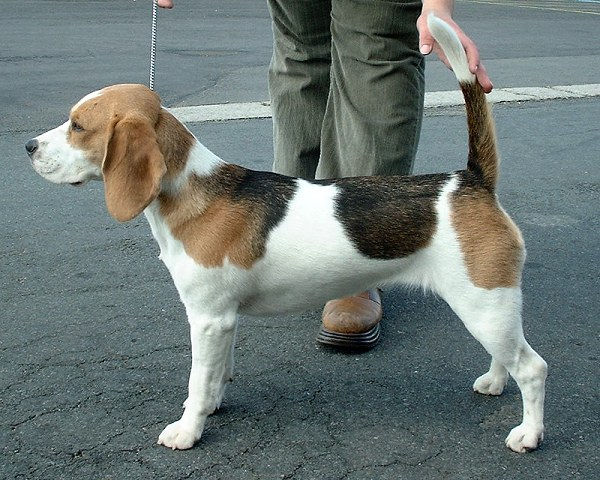
\includegraphics[width=0.9\linewidth]{Billeder/Jagthunde/stoevende/beagle.jpg} % Ikon af en drivende hund (f.eks. Beagle)

\end{columns}

\end{frame}